\documentclass[]{beamer}

% File: preamble.tex

\usepackage{lmodern}

% \usepackage{CJKutf8}
\usepackage{xeCJK}
\usetheme{CambridgeUS} % try Pittsburgh
\usecolortheme{beaver}
\usefonttheme[]{serif} % try "professionalfonts"

\setbeamertemplate{itemize items}[default]
\setbeamertemplate{enumerate items}[default]

\usepackage{animate}
\usepackage{xmpmulti}

% \usepackage{cancel, ulem}

\usepackage{amsmath, amsfonts, latexsym, mathtools, tabu}
\usepackage{centernot}
\newcommand{\z}{\mathbb{Z}}

\usepackage{amstext} % for \text macro
\usepackage{array}   % for \newcolumntype macro
\newcolumntype{C}{>{$}c<{$}} % math-mode version of "l" column type

\newcommand{\set}[1]{\left\{#1\right\}}
\newcommand{\ps}[1]{\mathcal{P}(#1)}
\usepackage{bm}
\DeclareMathOperator*{\argmin}{\arg\!\min}
\DeclareMathOperator*{\E}{\mathbb{E}}

% colors
\newcommand{\red}[1]{\textcolor{red}{#1}}
\newcommand{\redoverlay}[2]{\textcolor<#2>{red}{#1}}
\newcommand{\green}[1]{\textcolor{green}{#1}}
\newcommand{\greenoverlay}[2]{\textcolor<#2>{green}{#1}}
\newcommand{\blue}[1]{\textcolor{blue}{#1}}
\newcommand{\blueoverlay}[2]{\textcolor<#2>{blue}{#1}}
\newcommand{\purple}[1]{\textcolor{purple}{#1}}
\newcommand{\cyan}[1]{\textcolor{cyan}{#1}}
\newcommand{\violet}[1]{\textcolor{violet}{#1}}
\newcommand{\brown}[1]{\textcolor{brown}{#1}}
\newcommand{\lgray}[1]{\textcolor{lightgray}{#1}}
\newcommand{\teal}[1]{\textcolor{teal}{#1}}

% colorded box
\newcommand{\rbox}[1]{\red{\boxed{#1}}}
\newcommand{\gbox}[1]{\green{\boxed{#1}}}
\newcommand{\bbox}[1]{\blue{\boxed{#1}}}
\newcommand{\pbox}[1]{\purple{\boxed{#1}}}

\usepackage[linewidth = 1pt, framemethod = TikZ]{mdframed}
\mdfsetup{frametitlealignment=\center}

% #1: color; #2: text
\newcommand{\hl}[2]{\fcolorbox{#1}{#1!50}{#2}}

\usepackage{pifont}
\usepackage{wasysym}

\newcommand{\pno}[1]{\textcolor{blue}{\scriptsize [Problem: #1]}}

\newcommand{\cmark}{\green{\ding{51}}}
\newcommand{\xmark}{\red{\ding{55}}}
%%%%%%%%%%%%%%%%%%%%%%%%%%%%%%%%%%%%%%%%%%%%%%%%%%%%%%%%%%%%%%
% for fig without caption: #1: width/size; #2: fig file
\newcommand{\fig}[2]{
  \begin{figure}[htp]
    \centering
      \includegraphics[#1]{#2}
  \end{figure}
}

\newcommand{\sym}{\textsl{Sym}}
\newcommand{\gen}[1]{\langle #1 \rangle}
\newcommand{\card}[1]{\lvert #1 \rvert}
\newcommand{\bcard}[1]{\big\lvert #1 \big\rvert}
\newcommand{\Bcard}[1]{\Big\lvert #1 \Big\rvert}

\usepackage{adjustbox}
\usepackage{tikz}
\usetikzlibrary{shapes}

\newcommand{\titletext}{What We Talk About \\ When We Talk About Isomorphism Theorems}
 
\newcommand{\thankyou}{
  \begin{frame}[noframenumbering]{}
    \fig{width = 0.55\textwidth}{figs/thankyou}
  \end{frame}
}


%%%%%%%%%%
\title[\titletext]{\titletext}
\subtitle{}

\author[Hengfeng Wei]{\large 魏恒峰}
% \titlegraphic{\includegraphics[height = 2.0cm]{figs/qrcode-ps-2017-1st.png}}
\institute{hfwei@nju.edu.cn}
\date{2017年11月06日}

\AtBeginSection[]{
  \begin{frame}[noframenumbering, plain]
    \frametitle{\titletext}
    \tableofcontents[currentsection, sectionstyle=show/shaded, subsectionstyle=show/show/hide]
  \end{frame}
}
%%%%%%%%%%
\begin{document}

\maketitle

%%%%%%%%%%%%%%%
\begin{frame}{}
  \centerline{\LARGE Permutations}

  \vspace{0.50cm}
  \fignocaption{width = 0.30\textwidth}{figs/rubiks-cube}
\end{frame}
%%%%%%%%%%%%%%%

%%%%%%%%%%%%%%%
\begin{frame}{}
  \begin{exampleblock}{DH 2.9: \# of Permutations}
    Prove that the number of permutations of $A_n = \set{1 \cdots n}$ is $n!$.
  \end{exampleblock}

  \vspace{0.60cm}
  \begin{columns}
    \pause
    \column{0.50\textwidth}
      \begin{enumerate}[(1)]
	\item The ``choosing from'' method:
      \end{enumerate}
      \fignocaption{width = 0.70\textwidth}{figs/4-permtree}
    \pause
    \column{0.50\textwidth}
      \begin{enumerate}[(1)]
	\setcounter{enumi}{1}
	\item The ``inserting into'' method:
      \end{enumerate}
      \fignocaption{width = 0.70\textwidth}{figs/4-permtree}
  \end{columns}

  \vspace{0.60cm}
  \pause
  \centerline{\Large Prove by mathematical induction on $n$.}
\end{frame}
%%%%%%%%%%%%%%%

%%%%%%%%%%%%%%%
\begin{frame}{}
  \begin{exampleblock}{DH 2.9: \# of Permutations}
    Prove that the number of permutations of $A_n = \set{1 \cdots n}$ is $n!$.
  \end{exampleblock}

  \vspace{0.60cm}
  \begin{proof}[Prove by mathematical induction on $n$.]

    \[
      P(n): \text{\# of permutations of } A_n = \set{1 \cdots n} \text{ is } n!
    \]

    \pause

    \begin{description}
      \item[B.S.] $P(1)$
      \item[I.H.] $P(n)$
      \item[I.S.] $P(n) \to P(n+1)$
	\begin{description}
	  \pause
	  \item[Choosing from]
	  \pause
	  \item[Inserting into]
	\end{description}
    \end{description}
  \end{proof}
\end{frame}
%%%%%%%%%%%%%%%

%%%%%%%%%%%%%%%
\begin{frame}{}
  \begin{exampleblock}{DH 2.11: Generate All Permutations}
    Design an algorithm which, given a positive integer $N$,
    produces all the permutations of $A_N$.
  \end{exampleblock}


\end{frame}
%%%%%%%%%%%%%%%

%%%%%%%%%%%%%%%
\begin{frame}{}
  \begin{exampleblock}{DH 2.10: Permutation Checking}
    \begin{itemize}
      \item An integer $n$
      \item An array of integers $P$ of length $n$
    \end{itemize}
    To check whether $P$ is a permutation of $1 \cdots n$?
  \end{exampleblock}

  \vspace{0.60cm}
  \pause

  \begin{columns}
    \pause
    \column{0.40\textwidth}
      \begin{itemize}
	\item Boolean array $[1 \cdots n]$
      \end{itemize}
    \pause
    \column{0.15\textwidth}
      \begin{itemize}
	\item Sort
      \end{itemize}
    \pause
    \column{0.45\textwidth}
      \begin{itemize}
	\item $\forall x: x \in [1 \cdots n]$
	\item check for duplication
      \end{itemize}
  \end{columns}
\end{frame}
%%%%%%%%%%%%%%%


% stack-permutation.tex

%%%%%%%%%%%%%%%
\begin{frame}{}
  \begin{center}
    {\LARGE Stackable Permutations}
  \end{center}
\end{frame}
%%%%%%%%%%%%%%%

%%%%%%%%%%%%%%%
\begin{frame}{}
  \begin{definition}[Stackable Permutations]
    \uncover<2->{
      \[
	\fbox{$\texttt{out} = (a_1, \cdots, a_n) \blue{\xleftarrow[\;X \;=\; \bot\;]{\;S \;=\; \emptyset\;}} \texttt{in} = (1, \cdots, n)$}
      \]
    }

    \fig{width = 0.65\textwidth}{figs/stack-perm-x}
  \end{definition}
\end{frame}
%%%%%%%%%%%%%%%

%%%%%%%%%%%%%%%
\begin{frame}{}
  \fig{width = 0.50\textwidth}{figs/stack-perm-x}

  \begin{center}
    \red{We can assume that $X$ is always blank.}
  \end{center}

  \pause
  \[
    \cyan{\texttt{read}} + \purple{\texttt{push}} \qquad
    \cyan{\texttt{read}} + \cyan{\texttt{print}}
  \]
  \[
    \purple{\texttt{pop}} + \cyan{\texttt{print}} \qquad
    \purple{\texttt{pop}} + \purple{\texttt{push}}
  \]
\end{frame}
%%%%%%%%%%%%%%%

%%%%%%%%%%%%%%%
\begin{frame}{}
  \begin{columns}
    \column{0.50\textwidth}
      \fig{width = 0.90\textwidth}{figs/stack-perm-x}
    \pause
    \column{0.50\textwidth}
      \fig{width = 0.80\textwidth}{figs/stack-perm-inout}
  \end{columns}

  \pause
  \vspace{0.40cm}
  \fig{width = 0.40\textwidth}{figs/stack-perm}
\end{frame}
%%%%%%%%%%%%%%%

%%%%%%%%%%%%%%%
\begin{frame}{}
  \begin{definition}[Stackable Permutations]
    \[
      \fbox{$\texttt{out} = (a_1, \cdots, a_n) \blue{\xleftarrow{\;S \;=\; \emptyset\;}} \texttt{in} = (1, \cdots, n)$}
    \]

    \fig{width = 0.50\textwidth}{figs/stack-perm}
  \end{definition}
\end{frame}
%%%%%%%%%%%%%%%

%%%%%%%%%%%%%%%
\begin{frame}{}
  \begin{exampleblock}{DH 2.12: Stackable Permutations}
    \begin{enumerate}[(a)]
      \item Show that the following permutations \emph{\blue{are}} stackable:
	\begin{enumerate}[(i)]
	  \item $(3, 2, 1)$
	  \item \textcolor{purple}{$(3, 4, 2, 1)$}
	  \item $(3, 5, 7, 6, 8, 4, 9, 2, 10, 1)$
	\end{enumerate}
    \end{enumerate}
  \end{exampleblock}

  \pause
  \vspace{0.50cm}
  \begin{columns}
    \column{0.50\textwidth}
      \fig{width = 0.80\textwidth}{figs/stack-perm}
    \column{0.50\textwidth}
      \fig{width = 0.80\textwidth}{figs/no-choice}
  \end{columns}
\end{frame}
%%%%%%%%%%%%%%%

%%%%%%%%%%%%%%%
\begin{frame}{}
  \begin{exampleblock}{DH 2.13: Stackable Permutations Checking Algorithm}
    To check whether a given permutation can be obtained by a stack.
  \end{exampleblock}

  \vspace{0.50cm}
  \begin{columns}
    \column{0.50\textwidth}
      \fig{width = 0.75\textwidth}{figs/stack-perm}
    \column{0.50\textwidth}
      % stack-perm-alg-no-fail.tex

\begin{algorithm}[H]
  \begin{algorithmic}[1]
    \Procedure{Stackable}{$out$}
      \ForAll{$a_j \in out$}
	\While{$\blue{\textsf{top}(S) \neq a_j}$}
	  \State \purple{$\textsf{Push}(in, S)$}
	\EndWhile
	\State \purple{$\textsf{Pop}(out, S)$}
      \EndFor
    \EndProcedure
  \end{algorithmic}
\end{algorithm}

  \end{columns}

  \pause
  \vspace{0.60cm}
  \begin{center}
    \red{\it $Q:$ What is wrong with \textsc{Stackable}?}
  \end{center}
\end{frame}
%%%%%%%%%%%%%%%

%%%%%%%%%%%%%%%
\begin{frame}{}
  \begin{exampleblock}{DH 2.13: Stackable Permutations Checking Algorithm}
    To check whether a given permutation can be obtained by a stack.
  \end{exampleblock}

  \vspace{0.50cm}
  \begin{columns}
    \column{0.40\textwidth}
      \fig{width = 0.85\textwidth}{figs/stack-perm}
    \column{0.60\textwidth}
      % stack-perm-alg-fail.tex

\begin{algorithm}[H]
  \begin{algorithmic}[1]
    \Procedure{Stackable}{$out$}
      \ForAll{$a_j \in out$}
	\While{$\blue{\textsf{top}(S) \neq a_j \land in \neq \emptyset}$}
	  \State \purple{$\textsf{Push}(in, S)$}
	\EndWhile

	\hStatex
	\If{\teal{$\textsf{top}(S) = a_j$}}
	  \State \purple{$\textsf{Pop}(out, S)$}
	\Else  \Comment{\cyan{$\textsf{top}(S) \neq a_j \land in = \emptyset$}}
	  \State \Return $F$
	\EndIf
      \EndFor

      \hStatex
      \State \Return $T$
    \EndProcedure
  \end{algorithmic}
\end{algorithm}

  \end{columns}
\end{frame}
%%%%%%%%%%%%%%%

%%%%%%%%%%%%%%%
\begin{frame}{}
  \begin{exampleblock}{DH 2.12: Stackable Permutations}
    \begin{enumerate}[(a)]
      \setcounter{enumi}{1}
    \item \red{\bf Prove} that the following permutations are \emph{\blue{not}} stackable:
	\begin{enumerate}[(i)]
	  \item $(3, 1, 2)$
	  \item $(4, 5, 3, 7, 2, 1, 6)$
	\end{enumerate}
    \end{enumerate}
  \end{exampleblock}

  \uncover<2->{
    \[
      (\red{3}, \red{1}, \red{2})
    \]

    \[
      (4, 5, 3, \red{7}, \red{2}, 1, \red{6})
    \]
  }

  \uncover<3->{
    \[
      \blue{\fbox{$\texttt{out} = \cdots a_i \cdots a_j \cdots a_k: i < j < k \land a_j < a_k < a_i$}}
    \]
  }

  \uncover<4->{
    \[
      312\text{-Pattern}
    \]
  }
\end{frame}
%%%%%%%%%%%%%%%

%%%%%%%%%%%%%%%
\begin{frame}{}
  \begin{theorem}[Stackable Permutations]
    A permutation $(a_1, \cdots, a_n)$ is stackable $\iff$ it is not the case that
    \[
      312\text{\it -Pattern}: \fbox{$\texttt{\it out} = \cdots a_i \cdots a_j \cdots a_k: i < j < k \land a_j < a_k < a_i$}
    \]
  \end{theorem}

  \vspace{0.30cm}
  \pause
  \begin{proof}
    \begin{columns}
      \column{0.45\textwidth}
        \[
	  \blue{\text{stackable} \Longrightarrow \nexists \;312\text{-Pattern}}
        \]
	\uncover<3->{
	  \[
	    \red{312\text{-Pattern} \Longrightarrow \text{non-stackable}}
	  \]
	}
      \column{0.45\textwidth}
        \[
          \blue{\nexists \;312\text{-Pattern} \Longrightarrow \text{stackable}}
        \]
	\uncover<4->{
	  \[
	    \red{\exists \;\text{algorithm}}
	  \]
	}
    \end{columns}
  \end{proof}
\end{frame}
%%%%%%%%%%%%%%%

%%%%%%%%%%%%%%%
\begin{frame}{}
  \begin{theorem}[Stackable Permutations]
    A permutation $(a_1, \cdots, a_n)$ is stackable $\iff$ it is not the case that
    \[
      312\text{\it -Pattern}: \fbox{$\texttt{\it out} = \cdots a_i \cdots a_j \cdots a_k: i < j < k \land a_j < a_k < a_i$}
    \]
  \end{theorem}

  \vspace{0.30cm}
  \begin{proof}[$312\text{-Pattern} \Longrightarrow \text{non-stackable}$]
    \begin{columns}
      \column{0.17\textwidth}
      \column{0.65\textwidth}
        \pause
	\begin{description}[$j < k \land a_j < a_k$:]
	  \item[$i < j \land a_j < a_i$:] $\textsf{Push}_{j} \quad \textsf{Push}_{i} \quad \textsf{Pop}_{i} \quad \textsf{Pop}_{j}$
	  \item[$j < k \land a_j < a_k$:] $\textsf{Push}_{j} \quad \textsf{Pop}_{j} \quad \textsf{Push}_{k} \quad \textsf{Pop}_{k}$
	  \item[$i < k \land a_k < a_i$:] $\textsf{Push}_{k} \quad \textsf{Push}_{i} \quad \textsf{Pop}_{i} \quad \textsf{Pop}_{k}$
	\end{description}
      \column{0.17\textwidth}
    \end{columns}
  \end{proof}
\end{frame}
%%%%%%%%%%%%%%%

%%%%%%%%%%%%%%%
\begin{frame}[fragile]{}
  \begin{theorem}[Stackable Permutations]
    A permutation $(a_1, \cdots, a_n)$ is stackable $\iff$ it is not the case that
    \[
      312\text{\it -Pattern}: \fbox{$\texttt{\it out} = \cdots a_i \cdots a_j \cdots a_k: i < j < k \land a_j < a_k < a_i$}
    \]
  \end{theorem}

  \begin{proof}[$\nexists \;312\text{-Pattern} \Longrightarrow \text{Obtainable by \textsc{Stackable}}$]

    \uncover<2->{
      \begin{center}
	\red{\textsc{Stackable} fails $\implies \exists \;312\text{-Pattern}$.}
      \end{center}
    }

    \vspace{-0.50cm}
    \begin{columns}
      \column{0.60\textwidth}
        % stack-perm-alg-fail.tex

\begin{algorithm}[H]
  \begin{algorithmic}[1]
    \Procedure{Stackable}{$out$}
      \ForAll{$a_j \in out$}
	\While{$\blue{\textsf{top}(S) \neq a_j \land in \neq \emptyset}$}
	  \State \purple{$\textsf{Push}(in, S)$}
	\EndWhile

	\hStatex
	\If{\teal{$\textsf{top}(S) = a_j$}}
	  \State \purple{$\textsf{Pop}(out, S)$}
	\Else  \Comment{\cyan{$\textsf{top}(S) \neq a_j \land in = \emptyset$}}
	  \State \Return $F$
	\EndIf
      \EndFor

      \hStatex
      \State \Return $T$
    \EndProcedure
  \end{algorithmic}
\end{algorithm}

      \column{0.50\textwidth}
      \uncover<3->{
	\[
	  a_j \neq \textsf{top}(S) \land in = \emptyset 
	\]
      }
      \vspace{-0.30cm}
      \uncover<4->{
	\[
	  \red{\it a_j \text{ is covered by some } a_k \text{ in } S}
	\]
      }
      \vspace{-0.30cm}
      \uncover<5->{
	\[
	 \exists k: j < k \land a_j < a_k
	\]
      }
      \vspace{-0.30cm}
      \uncover<6->{
	\[
	  \red{\it \text{Why is } a_k \text{ in } S?}
	\]
      }
      \vspace{-0.30cm}
      \uncover<7->{
	\[
	 \exists i: i < j \land a_k < a_i
	\]
      }
    \end{columns}
  \end{proof}
\end{frame}
%%%%%%%%%%%%%%%

%%%%%%%%%%%%%%%
\begin{frame}{}
  \begin{exampleblock}{DH 2.12: Stackable Permutations}
    \begin{enumerate}[(a)]
      \setcounter{enumi}{2}
      \item How many permutations of $A_4$ \red{\emph{cannot}} be obtained by a stack?
    \end{enumerate}
  \end{exampleblock}

  \begin{align*}
    &(1, \redoverlay{4}{2-}, \redoverlay{2}{2-}, \redoverlay{3}{2-}), (2, 4, 1, 3), (3, 1, 2, 4), 
    (\redoverlay{3}{2-}, \redoverlay{1}{2-}, 4, \redoverlay{2}{2-}), (3, 4, 1, 2) \\
    &(4, 1, 2, 3), (4, 1, 3, 2), (\redoverlay{4}{2-}, 2, \redoverlay{1}{2-}, \redoverlay{3}{2-}), (4, 2, 3, 1), (4, 3, 1, 2)
  \end{align*}

  \vspace{0.60cm}
  \uncover<3->{
    \begin{center}
      {\red{\it $Q:$ What about $A_n$?}}
    \end{center}
  }
\end{frame}
%%%%%%%%%%%%%%%

%%%%%%%%%%%%%%%
\begin{frame}{}
  \begin{exampleblock}{DH 2.12: Stackable Permutations}
    How many permutations of $\set{1 \cdots n}$ are stackable?
  \end{exampleblock}

  \fig{width = 0.50\textwidth}{figs/stack-perm}

  \pause
  \centerline{\red{$Q:$} How many \blue{\emph{admissible}} operation sequences of \purple{``\texttt{Push}''} and \purple{``\texttt{Pop}''}?}
\end{frame}
%%%%%%%%%%%%%%%

%%%%%%%%%%%%%%%
\begin{frame}{}
  \begin{definition}[Admissible Operation Sequences]
    An operation sequence of \purple{``\texttt{Push}''} and \purple{``\texttt{Pop}''} is \blue{\it admissible} if and only if
    \begin{enumerate}[(i)]
      \pause
      \item $\# \text{ of ``\texttt{Push}''} = n \qquad \# \text{ of ``\texttt{Pop}''} = n$
      \pause
      \item $\forall \text{ prefix}: (\# \text{ of ``\texttt{Pop}''}) \le (\# \text{ of ``\texttt{Push}''})$
    \end{enumerate}
  \end{definition}

  \vspace{0.50cm}
  \pause
  \begin{center}
    \red{\fbox{\# of admissible operation sequences $=$ \# of stackable perms}}
  \end{center}

  \pause
  \[
    \set{\text{admissible operation sequences}} \xrightarrow{\exists f: 1-1} \set{\text{stackable perms}}
  \]

  \pause
  \[
    f(s) \triangleq \text{\red{\it Execute} this admissible operation sequence } s
  \]

  \pause
  \begin{center}
    \red{\it Why is $f$ bijective (1-1)?}
  \end{center}
\end{frame}
%%%%%%%%%%%%%%%

%%%%%%%%%%%%%%%
% \begin{frame}{}
%   \begin{theorem}
%     Different admissible operation sequences correspond to different permutations.
%   \end{theorem}
% 
%   \vspace{0.30cm}
%   \pause
%   \begin{proof}
%     \begin{align*}
%       &\push{}\; \;\push{}\; \;\push{}\; \;\pop{}\; \;\pop{}\; \;\red{\push{}} \cdots \\
%       &\push{}\; \;\push{}\; \;\push{}\; \;\pop{}\; \;\pop{}\; \;\red{\pop{}} \cdots \\
%     \end{align*}
%   \end{proof}
% \end{frame}
%%%%%%%%%%%%%%%

%%%%%%%%%%%%%%%
\begin{frame}{}
  \begin{theorem}
    The number of admissible operation sequences of \texttt{\it \purple{``Push''}} and \texttt{\it \purple{``Pop''}} is ${2n \choose n} - {2n \choose n-1}$.
  \end{theorem}

  \pause
  \begin{proof}[Proof: The Reflection Method]
    \[
      \push{}: \;\rightarrow \qquad \pop{}: \;\uparrow
    \]

    \begin{columns}
      \pause
      \column{0.50\textwidth}
	% \fig{width = 0.90\textwidth}{figs/grid-path}
	\begin{center}
	  \resizebox{0.80\textwidth}{!}{\input{tikz/grid}}
	\end{center}
      \column{0.50\textwidth}
	\uncover<6->{
	  \[
	    \blue{\underbrace{\textcolor{black}{{2n \choose n}}}_{\text{all}}} 
	    - \red{\underbrace{\textcolor{black}{{2n \choose n-1}}}_{\text{inadmissible}}}
	  \]
	}
    \end{columns}
  \end{proof}
\end{frame}
%%%%%%%%%%%%%%%

%%%%%%%%%%%%%%%
\begin{frame}{}
  \begin{center}
    \resizebox{0.60\textwidth}{!}{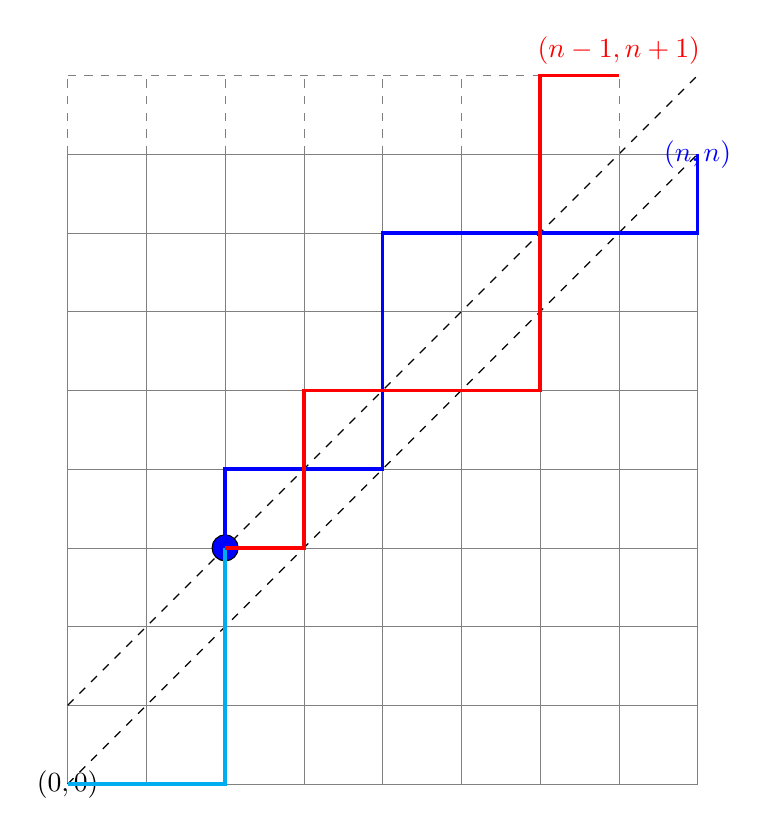
\begin{tikzpicture}
  \draw[help lines] (0,0) grid (8,8);

  \node (00) [] {$(0,0)$};
  \node (01) [] at (0,1) {};
  \node (nn) [blue] at (8,8) {$(n,n)$};

  \draw [dashed] (0,0) to (8,8);

  \pause
  \draw[very thick] (0,0) -- (1,0) -- (2,0) --
	(2,1) -- (2,2) -- (2,3);
  \draw[very thick] (2,3) -- (2,4) --
	(3,4) -- (4,4) --
	(4,5) -- (4,6) -- (4,7) --
	(5,7) -- (6,7) -- (7,7) -- (8,7) --
	(8,8);

  \pause
  \node (nn1) [] at (8,9) {};
  \draw [dashed] (0,1) to (8,9);

  \pause
  \node () [circle, draw, fill = blue] at (2,3) {};

  \pause
  \draw[very thick, cyan] (0,0) -- (1,0) -- (2,0) --
	(2,1) -- (2,2) -- (2,3);
  \draw[very thick, blue] (2,3) -- (2,4) --
	(3,4) -- (4,4) --
	(4,5) -- (4,6) -- (4,7) --
	(5,7) -- (6,7) -- (7,7) -- (8,7) --
	(8,8);

  \pause
  \draw[help lines, dashed] (0,8) grid (7,9);
  \draw[very thick, red] 
	(2,3) -- (3,3) --
	(3,4) -- (3,5) --
	(4,5) -- (5,5) -- (6,5) --
	(6,6) -- (6,7) -- (6,8) -- (6,9) --
	(7,9) node[above] () {$(n-1, n+1)$};
\end{tikzpicture}}
  \end{center}
\end{frame}
%%%%%%%%%%%%%%%

%%%%%%%%%%%%%%%
% \begin{frame}{}
%   \begin{center}
%     \resizebox{0.60\textwidth}{!}{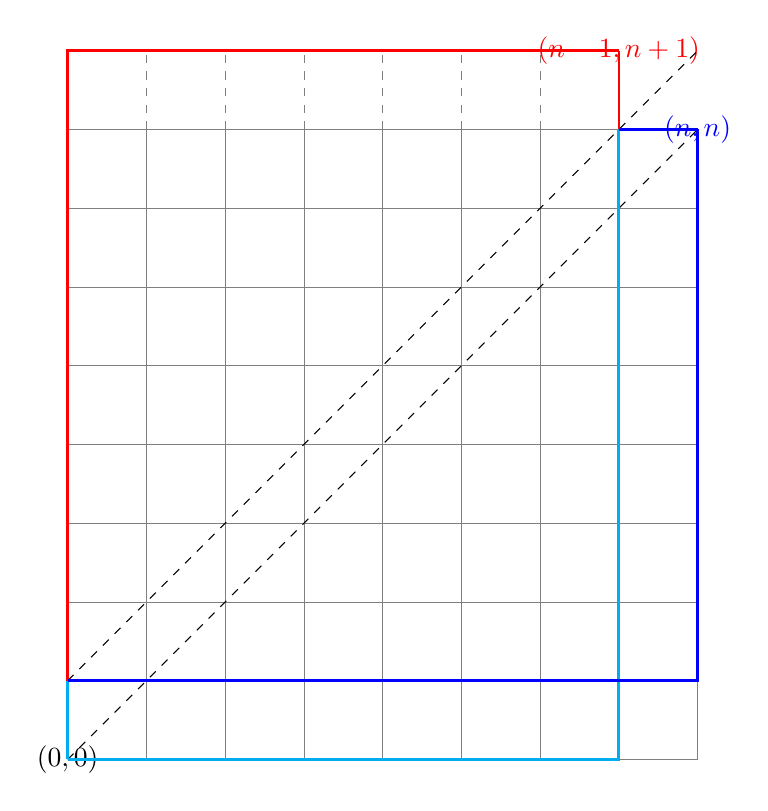
\begin{tikzpicture}
  \draw[help lines] (0,0) grid (8,8);
  \draw[help lines, dashed] (0,8) grid (7,9);

  \node (00) [] {$(0,0)$};
  \node (01) [] at (0,1) {};
  \node (nn) [blue] at (8,8) {$(n,n)$};
  \node (nn1) [] at (8,9) {};
  \node (n1n1) [red] at (7,9) {$(n-1, n+1)$};

  \draw [dashed] (0,0) to (8,8);
  \draw [dashed] (0,1) to (8,9);

  \uncover<2-3>{
    \draw[very thick, cyan] (0,0) -- (7,0) -- (7,8);
  \draw[thick, red] (7,8) -- (7,9);
  }
  \uncover<3>{
    \draw[very thick, blue] (7,8) -- (8,8);
  }

  \uncover<4-5>{
    \draw[very thick, cyan] (0,0) -- (0,1);
    \draw[very thick, red] (0,1) -- (0,9) -- (7,9);
  }
  \uncover<5>{
    \draw[very thick, blue] (0,1) -- (8,1) -- (8,8);
  }
\end{tikzpicture}
}
%   \end{center}
% \end{frame}
%%%%%%%%%%%%%%%

%%%%%%%%%%%%%%%
\begin{frame}{}
  \[
    {2n \choose n} - {2n \choose n-1}
  \]

  \begin{center}
    {\Large \href{https://en.wikipedia.org/wiki/Catalan\_number}{Catalan Number}}
  \end{center}

  \[
    (3,2,1): ((())) \qquad (1,2,3): ()()()
  \]
\end{frame}
%%%%%%%%%%%%%%%
%%%%%%%%%%%%%%%
\begin{frame}{}
  \centerline{\LARGE Treesort Algorithm on BST}

  \vspace{0.30cm}
  \fig{width = 0.35\textwidth}{figs/bst}
\end{frame}
%%%%%%%%%%%%%%%

%%%%%%%%%%%%%%%
\begin{frame}{}
  \begin{columns}
    \column{0.48\textwidth}
      % build-bst.tex

\begin{algorithm}[H]
  \begin{algorithmic}[1]
    \Procedure{BuildBST}{$eles$}
      \State \textsl{Node} $root(eles[0])$

      \Statex
      \ForAll{$e \in eles[1 \ldots]$}
	\State \Call{insert}{$root, e$}
      \EndFor
    \EndProcedure
  \end{algorithmic}
\end{algorithm}

    \column{0.53\textwidth}
      % bst-insert.tex

\begin{algorithm}[H]
  \begin{algorithmic}[1]
    \Procedure{Insert}{$T$, $e$}
      \If{\red{$e < T.val$}}
	\If{$T.left = \Lambda$}
	  \State $T.left = \textsl{new Node}(e)$
	\Else
	  \State \blue{\Call{Insert}{$T.left, e$}}
	\EndIf
      \Else 
	\If{$T.right = \Lambda$}
	  \State $T.right = \textsl{new Node}(e)$
	\Else
	  \State \blue{\Call{Insert}{$T.right, e$}}
	\EndIf
      \EndIf
    \EndProcedure
  \end{algorithmic}
\end{algorithm}

  \end{columns}
\end{frame}
%%%%%%%%%%%%%%%

%%%%%%%%%%%%%%%
% \begin{frame}[fragile]{}
%   \begin{lstlisting}[style = Cstyle]
%   procedure |\purple{put x into a BST t}|:
%     ... call |\purple{put x into t$'$s left subtree}|
%     ... call |\purple{put x into t$'$s right subtree}|
%   end procedure
%   \end{lstlisting}
% 
%   \pause
%   \vspace{0.30cm}
%   \centerline{\red{\Large should be:}}
%   \vspace{0.20cm}
%   \begin{lstlisting}[style = Cstyle]
%   procedure |\purple{put-x-into-BST}| (t):
%     ... call |\purple{put-x-into-BST}| (t$'$s left subtree)
%     ... call |\purple{put-x-into-BST}| (t$'$s right subtree)
%   end procedure
%   \end{lstlisting}
% \end{frame}
%%%%%%%%%%%%%%%

%%%%%%%%%%%%%%%
\begin{frame}[fragile]{}
  \begin{exampleblock}{DH 2.16: Treesort}
    \begin{enumerate}[(i)]
      \setcounter{enumi}{1}
      \item right; \quad val; \quad left
    \end{enumerate}
  \end{exampleblock}

  \vspace{0.30cm}
  \fig{width = 0.35\textwidth}{figs/bst}

  \pause
  \[
    14,\quad 13,\quad 10,\quad 8,\quad 7,\quad 6,\quad 4,\quad 3,\quad 1
  \]
\end{frame}
%%%%%%%%%%%%%%%


\thankyou{}

\end{document}
%%%%%%%%%%